\documentclass[a4paper, 14pt]{article}
\usepackage{pre}


\begin{document}
    % Оформление титульного листа
\begin{titlepage}
    \newpage
    
    \begin{center}
    МИНИСТЕРСТВО НАУКИ И ВЫСШЕГО ОБРАЗОВАНИЯ РОССИЙСКОЙ ФЕДЕРАЦИИ ФЕДЕРАЛЬНОЕ ГОСУДАРСТВЕННОЕ АВТОНОМНОЕ ОБРАЗОВАТЕЛЬНОЕ УЧРЕЖДЕНИЕ ВЫСШЕГО ОБРАЗОВАНИЯ НАЦИОНАЛЬНЫЙ ИССЛЕДОВАТЕЛЬСКИЙ ЯДЕРНЫЙ УНИВЕРСИТЕТ «МИФИ» \\
    \end{center}
    
    
    \vspace{2.5em} % Делаем вертикальный пробел в 3em
    
    \begin{center}
        \textsc{\textbf{Кафедра теоретической ядерной физики\\}}
    \end{center}
    \vspace{1em}
    \begin{center}
    \textsc{На правах рукописи\\} 
    \end{center}
    \begin{center}
        \textsc{\Large Широков Денис Дмитриевич\linebreak  \linebreak  \Large \textbf{ <<Численные методы решения задач математической физики с использованием локально-адаптивных сеток>>}}
    \end{center} 
    
    \vspace{1em}
    
    \begin{center}
    Выпускная квалификационная работа бакалавра \linebreak Направление подготовки 03.03.01 Прикладные математика и физика
    \end{center}
    
    \vspace{1em}
    
   
    \newbox{\lbox}
    \savebox{\lbox}{\hbox{Широков Денис Дмитриевич}}
    \newlength{\maxl}
    \setlength{\maxl}{\wd\lbox}
    \hfill\parbox{9cm}{
    \hspace*{1.5cm}\hspace*{-3cm}Выпускная квалификационная\\ \hspace*{1.5cm}\hspace*{-3cm}работа защищена\\ 
    
    \hspace*{1.5cm}\hspace*{-3cm}<<\rule{1.5em}{1pt}>>\hbox to\maxl{\rule{6em}{1pt}2021 г.\hfill}\\
    
    \hspace*{1.5cm}\hspace*{-3cm}Оценка \hbox to\maxl{\rule{7em}{1pt}\hfill}\\
    
    \hspace*{1.5cm}\hspace*{-3cm}Секретарь ГЭК 
    \hbox to\maxl{\rule{5em}{1pt} Фамилия И.О.\hfill}\hfill\\  
    \hspace*{7.0cm}\hspace*{-3cm}к.ф.-м.н., доцент\hfill\\
    
    }
    
    

    
    
    \vspace{\fill}
    
    \begin{center}
    \textbf{Москва}\\
    \today
    \end{center}

\end{titlepage}

    % Оформление титульного листа
\begin{titlepage}
    \newpage
    
    \vspace{3em} % Делаем вертикальный пробел в 3em
    
   
    \begin{center}
        \textsc{ \textbf{Пояснительная записка\linebreak к бакалаврской дипломной работе: \linebreak  \Large <<Численное решение уравнения теплопроводности с использованием локально-адаптивных сеток>>}}
    \end{center} 

    
    \vspace{5em}
    
   
    \newbox{\lbox}
    \savebox{\lbox}{\hbox{Широков Денис Дмитриевич}}
    
    \setlength{\maxl}{\wd\lbox}
    \hfill\parbox{12cm}{
    \hspace*{1cm}\hspace*{-1cm}Студент\hfill\hbox to\maxl{\rule{5em}{1pt} Широков Д.Д.\hfill}\\
    
    \hspace*{1cm}\hspace*{-1cm}Научный руководитель\hfill\\
    \hspace*{1cm}\hspace*{-1cm}к.ф.-м.н.\hfill\hbox to\maxl{\rule{5em}{1pt} Кучугов П.А.\hfill}\\ \\
    \hspace*{1cm}\hspace*{-1cm}Рецензент\hfill\\
    \hspace*{1cm}\hspace*{-1cm}к.ф.-м.н.\hfill\hbox to\maxl{\rule{5em}{1pt} Ладонкина М.Е. \hfill}\\ \\ 
    \hspace*{1cm}\hspace*{-1cm}Заведующий кафедрой \hfill\\
    \hspace*{1cm}\hspace*{-1cm}к.ф.-м.н.\hfill\hbox to\maxl{\rule{5em}{1pt} Муравьев С.Е. \hfill}\\ \\ 
    
    }
    
   
    
    


\end{titlepage}


    % Аннотация
    \section*{Аннотация}
    В работе проведён подробный анализ численного метода разностных схем решения уравнения теплопроводности, исследуются преимущества и недостатки использования равномерных статических сеток в случае квазилинейных уравнений с существенно различающимися масштабами (как пространственными, так и временными) физическими процессами.
Разработано программное обеспечение, реализующее рассмотренные схемы численного решения, проверены описанные особенности каждой и схем.
Показана необходимость использования сеток с локальным измельчением, подстраивающееся под особенности решения.
Описаны некоторые теоретические основы данного метода.
Реализован в виде программного кода соответствующий алгоритм, работоспособность которого проверена на нескольких тестовых задачах.
Показаны преимущества использования блочных локально-адаптивных сеток по сравнению с использованием равномерных статических.
    \newpage

    % Содержание
    \tableofcontents
    \newpage

    % Введение
    \section{Введение}
    Здесь будет введение

    % Основные понятия теории разностных схем
    \section{Основные понятия теории разностных схем}\label{sec:MainDiffSchemes}
    Математическая формулировка физических задач, описанных во введении имеет вид:
\begin{equation}\label{eq:InitialProblem}
    \begin{cases}
        L[u](x) = f(x), & x = (x_1, \ldots, x_n)^{T} \in G \subset \mathbb{R}^n\\
        \Gamma[u](x) = \mu(x), & x \in \partial G
    \end{cases}, 
\end{equation}
где 
\begin{itemize}
    \item $L$~--- дифференциальный оператор уравнения;
    \item $\Gamma$~--- оператор начально-краевых условий (в общем случае также дифференциальный);
    \item $f$, $\mu$~--- заданные функции.
\end{itemize}
Решения исходной задачи~--- функции $u(x)$ непрерывного аргумента $x \in G$, являются элементами некоторого функционального пространства $H_0$ с нормой $\norm{\cdot}$.
В методе конечных разностей область $G$ заменяется на некоторое дискретное множество точек $\omega_h$, именуемое \emph{сеткой}, а функциональное пространство $H_0$ заменяется на $H_h$~--- гильбертово пространство сеточных функций ${y_h : G \supset \omega_h \rightarrow \mathbb{R}}$, где $h$~--- некоторый параметр, характеризующий сетку $\omega_h$ в области $G$.
Например, равномерная статическая сетка:
\begin{equation*}
    \omega_h = \{x = (x_1, \ldots, x_n) \in G \mid x_i = h_i \cdot k,\,\, k = 0, 1, \ldots, N_i\,\, i = 1, \ldots, n\}
\end{equation*}
Получив приближённое решение задачи $y_h$, необходимо оценивать степень \glqq близости\grqq к решению исходной задачи $u(x)$.
$y_h$~и~$u$ являются элементами разных функциональных пространств, поэтому для оценивания близости в работе используется проекционный метод: пространство $H_0$ отображается (проектируется) на пространство $H_h$ оператором $\mathcal{P}$:
\begin{equation*}
    \mathcal{P}_h \colon H_0 \ni u \mapsto u_h \in H_h.
\end{equation*}
Простейший выбор: ограничение $u$ на сетку $\omega_h$:
\begin{equation*}
    u_h(x) := u(x),\quad x \in \omega_h \subset G
\end{equation*}
Иногда пользуются \glqq более равномерным\grqq способом ограничения с усреднением по окрестности узла:
\begin{equation*}
    u_h(x) := \frac{1}{2h} \int_{x - h}^{x + h} u(x') dx'
\end{equation*}
Тогда близость приближённого решения $y_h$ и исходного решения $u$ оценивается по норме $\norm{\cdot}_{h}$ пространства $H_h$:
\begin{equation*}
    e = \norm{y_h - u_h}_{h},
\end{equation*}
при этом требуется, чтобы она аппроксимировала норму $\norm{\cdot}_{0}$ в слудеющем смысле\cite{СамарскийТеорияРазностныхСхем}:
\begin{equation*}
    \lim\limits_{h \rightarrow 0} \norm{u_h}_h = \norm{u}_{0}
\end{equation*}
В работе используется норма
$
    \norm{y}_{h} = \sqrt{
        \sum_{i=1}^{N} hy_i^2
    }
$.
Исходному дифференциальному оператору $L$ ставится в соответствие \emph{разностный оператор} $L_h$:
\begin{equation*}
    L_h[v] (x) = \sum_{x' \in T(x)} A_h(x, x') v(x'),
\end{equation*}
где $T(x)$~--- некоторое множество узлов сетки, называемое \emph{шаблоном}.
Например, двумерный оператор Лапласа $L = \Delta$ на двумерной равномерной сетке можно аппроксимировать, используя шаблон \glqq крест\grqq (\seefigref{fig:cross}):
\begin{equation*}
    \Delta u(x) = \frac{\partial^2 u}{\partial x_1^2} + \frac{\partial^2 u}{\partial x_2^2} \mapsto 
    \frac{u_{i+1}^{j} - 2u_{i}^{j} + u_{i-1}^j}{h_1^2} +
    \frac{u_i^{j + 1} - 2u_i^{j} + u_i^{j-1}}{h_2^2}, 
\end{equation*}
где $u_i^j = u({x_1}_i, {x_2}_j),\quad ({x_1}_i, {x_2}_j) \in \omega_h$.
\begin{figure}
    \centering
    \begin{tikzpicture}
        \filldraw[black] (0, 0) circle(2pt) node[anchor=south west] {$(x_1, x_2)$};
        \draw (-2.5, 0) node[anchor=north] {$(x_1 - h_1, x_2)$} -- (2.5, 0) node[anchor=north] {$(x_1 + h_1, x_2)$};
        \filldraw[black] (-2.5, 0) circle(2pt);
        \filldraw[black] (2.5, 0) circle(2pt);
        \filldraw[black] (0, -2.5) circle(2pt);
        \filldraw[black] (0, 2.5) circle(2pt);
        \draw (0, -2.5) node[anchor=north] {$(x_1, x_2 - h_2)$} -- (0, 2.5) node[anchor=south] {$(x_1, x_2 + h_2)$};
    \end{tikzpicture}
    \caption{Шаблон \glqq Крест\grqq}
    \label{fig:cross}
\end{figure}
Погрешность аппроксимации оператора $L$ разностным оператором $L_h$ определяется как сеточная функция $\psi_h = L_h[u_h] - (L[u])_h, u \in H_0$.
Если $\norm{\psi_h} = O(|h|^m)$, то говорят, что оператор $L_h$ аппроксимирует оператор $L$ с порядком $m$.
Если $\psi(x) = O(h^m), m$, то говорят, что оператор $L_h$ аппроксимирует оператор $L$ в точке $x$ с порядком $m$.

Теперь сформулируем непосредственно то, что называется \emph{разностной схемой}, алгоритмы решения которой и реализуются на компьютере.
Исходной задаче \eqref{eq:InitialProblem} ставится в соответствие семейство разностных задач, зависящих от параметра $h$, называемое разностной схемой:
\begin{equation*}
    \left\{ 
        \begin{cases}
            L_h [y_h] = \phi_h, & x \in \omega_h\\
            l_h [y_h] = \chi_h, & x \in \gamma_h
        \end{cases}
     \right\}_h,\quad \phi_h = \mathcal{P}_h[f], \chi_h = \mathcal{P}_h[\mu]
\end{equation*}
Под погрешностью разностной схемы понимается $z_h = y_h - u_h$, где $u_h = \mathcal{P}_h u$~--- проекция решения исходной задачи на $H_0$. 
Решения разностной задачи сходится к решению исходной задачи, если 
\begin{equation*}
    \norm{z_h}_{h} \rightarrow 0 \text{ при } |h| \rightarrow 0
\end{equation*}
Введём также понятие устойчивости схемы.
Разностная схема называется устойчивой (корректной, сходящейся), если
$
    \exists h_0 > 0 : \forall h(|h| \le h_0) \Rightarrow
$
\begin{equation*}
    \begin{aligned}
        &1. \forall \phi \in H_h \quad \exists! y_h\text{--- решение};\\
        &2. \exists M > 0 : \forall \phi_h, \tilde{\phi}_h \norm{y_h - \tilde{y}_h} \le M \norm{\phi_h - \tilde{\phi}_h}
    \end{aligned}
\end{equation*}

На этом только лишь математическая сторона вопроса формулирования проблемы завершена. 
Дальнейшие шаги по исследованию разностной схемы опираются на конкретный выбор множества сеток $\left\{ \omega_h \right\}$ и аппроксимирующего оператора $L_h$, выбор которого, в свою очередь, существенно зависит от некоторых вопросов реализации получаемого алгоритма на компьютере.







% например, в случае квазилинейного уравнения теплопроводности
% $
%     L = \frac{\partial }{\partial t} - 
%     \sum\limits_{i = 1}^{n} \frac{\partial }{\partial x_i} \left( 
%         k(x) \frac{\partial u}{\partial x_i}
%      \right)
% $;

% Сетки и сеточные функции
% Пусть $H_0$~--- некоторое функциональное пространство функций $u(x)$ непрерывного аргумента $x \in G$ с нормой $\|\cdot\|_0$.
% В методе конечных разностей область $\bar{G}$ изменения аргумента $x$ заменяется сеткой $\bar{\omega}_h$~--- конечным множеством точек $x_i \in \bar{G}$,
% а функциональное пространство $H_0$ заменяется на $H_h$~--- гильбертово пространство сеточных функций $y_h(x)$, определённых на сетке $\bar{\omega}_h$ с нормой $\|\cdot\|_h$.
% Обычно будем пользоваться нормой $\|y\|_h = \left( \sum\limits_{i = 1}^{N} h y_i^2 \right)^{1/2}$
% Функции $y_h(x) \in H_h$~--- численные решения, аппроксимации исходных решений $u(x) \in H_0$.
% Соответственно, основной интерес теории приближённых методов представляет \textbf{оценка близости} $y_h$ к $u$.
% Эти два вектора являются элементами разных пространств. Их близость описываем следующим образом:

% $\mathcal{P}_h: H_0 \rightarrow H_h,\quad u \mapsto u_h: u_h(x) = u(x), x \in \bar{\omega}_h$.
% Тогда близость $u_h$ и $y_h$ характеризуется числом $\|y_h - u_h\|_h$.

% Условие согласования норм в $H_h$ и $H_0$:
% $\lim\limits_{h \rightarrow 0} \|u_h\|_h = \| u\|_0$, или другими словами "норма $\|\cdot\|_h$ аппроксимирует норму $\|\cdot\|_0$"


% Разностная аппроксимация дифференциальных операторов

% Пусть $L$~--- линейный дифференциальный оператор, $\mathcal{D}(L) = H_0$, $\quad Ш(x) \subset \bar{\omega}_h$~--- некоторое множество узлов сетки

% \textbf{Опр.} $L_h v_h (x) = L_h v_h(x) = \sum\limits_{\xi \in Ш(x)} A_h(x, \xi) v_n (\xi)$~--- разностный оператор, разностная аппроксимация оператора $L$

% \textbf{Опр.} $\psi(x) = L_h v(x) - L v(x)$~--- локальная погрешность разностной аппроксимации $Lv$ в точке $x$.

% \textbf{Опр.} $L_h$ аппроксимирует $L$ с порядком $ m > 0$ в точке $x$, если $\psi(x) = L_h v(x) - Lv(x) = O(h^m)$

% \textbf{Опр.} Погрешность аппроксимации оператора $L$ разностным оператором $L_h$~--- это сеточная функция
% $\psi_h = L_h v_h - (Lv)_h, \quad (Lv)_h = \mathcal{P}_h (Lv), \quad v \in H_0$

% \textbf{Опр.} Разностный оператор $L_h$ аппроксимирует дифференциальный оператор $L$ с порядком $m>0$, если
% $$
%     \| \psi_h \| = \| L_h v_h - (Lv)_h \|_h = O(|h|^m)
% $$

% Общее утверждение, касательно аппроксимации дифференциальных операторов разностными таково, что:
% * погрешность аппроксимации зависит от используемого шаблона, причём можно достичь любого порядка локальной аппроксимации повышением кол-ва узлов шаблона (однако ухудшается качество операторов)
% * исследование локальной аппроксимации может оказаться недостаточным для суждения о порядке разностной аппроксимации на сетке и тем самым для суждения о качестве разностного оператора
% * рассмотрение разностной аппроксимации на решении дифференциального уравнения может использоваться для повышения порядка аппроксимации


% Постановка разностных задач.

% $G\subset \mathbb{R}^n$, $\partial G = \Gamma$, $L, l$~--- линейные дифференциальные операторы, $\mathcal{D}(L) = H_0$, $\mathcal{D}(l) = H_0$. 
% Исохдной задаче
% $$
%     \begin{cases}
%         Lu(x) = f(x), & x \in G\\
%         lu(x) = \mu (x), & x \in \Gamma
%     \end{cases}
% $$
% ставится в соответствие *семейство разностных задач*, зависящих от параметра $h$, называемое *разностной схемой*:
% $$
%     \left\{ 
%         \begin{cases}
%             L_h y_h = \varphi_h, & x \in \omega_h\\
%             l_h y_h = \chi_h, & x \in \gamma_h
%         \end{cases}
%         \right\}_h
% $$

% \textbf{Опр.} Погрешность разностной схемы $z_h = y_h - u_h$, где $y_h$~--- решение разностной задачи, а $u_h = \mathcal{P}_h u$ проекция решения исходной задачи на $H_0$.

% \textbf{Опр.} Погрешность аппроксимации для уравнения $L_h y_h = \varphi_h$ на решении $u(x)$ уравнения $Lu = f$:
% $$
%     \psi_h = L_h z_h = \varphi_h - L_h u_h
% $$
% погрешность аппроксимации для условия $l_h y_h = \chi_h$ на решении $u(x)$ исходной задачи:
% $$
%     \nu_h = l_h z_h = \chi_h - l_h u_h
% $$

% \textbf{Опр.} Решение разностной задачи *сходится к решению исходной задачи*, если 
% $$
%     \| z_h\|_h = \|y_h - u_h \|_h \rightarrow 0 \quad  |h| \rightarrow 0
% $$

% \textbf{Опр.} Разностная схема *сходится со скоростью* $O(|h|^m)$ (*имеет $m$-ый порядок точности*), если 
% $$
%     \| z_h \|_h = \| y_h - u_h \|_h = O(|h|^m), \quad |h| \rightarrow 0
% $$

% \textbf{Опр.} Разностная схема обладает $n$-ым порядком аппроксимации, если
% $$
%     \| \psi_h \|_h = O(|h|^n),\quad \| \nu_h \|_h = O(|h|^n)
% $$

% \textbf{Опр.} Разностная схема называется корректной (устойчивой, сходящейся), если
% $\exists h_0 > 0 : \forall h (|h| \leqslant h_0) \Rightarrow$
% 1. $\forall \varphi \in \tilde{H}_h \,\, \exists ! y_h$~--- решение;
% 2. $\exists M > 0 : \forall \varphi_h, \tilde{\varphi}_h \quad \| y_h - \tilde{y}_h \| \leqslant M \| \varphi_h - \tilde{\varphi}_h \|$

% **Утв.** Если схема устойчива и аппроксимирует исходную, т.е. $\| \psi_h \|_h = O(|h|^n)$, то она сходится, причём порядок сходимости совпадает с порядком аппроксимации.

    % Разностные схемы на статических сетках
    \section{Разностные схемы на статических сетках}\label{sec:StaticGrid}
        % Общие замечания
        Здесь будет введение

        % Избранные разностные схемы для ур-ния теплопроводности
        \subsection{Избранные разностные схемы для уравнения теплопроводности}
            % Явная схема
            \subsubsection{Явная схема}
            \begin{figure}[h]
    \centering
        \begin{tikzpicture}
            \filldraw[black] (0, 0) circle(2pt) node[anchor=south west] {$(x_i, t_j)$};
            \draw (-2.5, 0) node[anchor=north] {$(x_{i - 1}, t_j)$} -- (2.5, 0) node[anchor=north] {$(x_{i + 1}, t_j)$};
            \filldraw[black] (-2.5, 0) circle(2pt);
            \filldraw[black] (2.5, 0) circle(2pt);
            \filldraw[black] (0, 2.5) circle(2pt);
            \draw (0, 0) -- (0, 2.5) node[anchor=south]{$(x_i, t_{j + 1})$};
        \end{tikzpicture}
    \caption{Пятиточечный шаблон явной схемы}
    \label{fig:ExplicitTemplate}
\end{figure}
Шаблон явной схемы нагляден в одномерном случае (\seefigref{fig:ExplicitTemplate}).
Множество $\{(x, t) \in \omega_h \mid t = t_j\}$ будем называть $j$--ым временным слоем.
Оператор $\frac{\partial u}{\partial t}$ аппроксимируется, используя значения функции на $(j + 1)$--ом временном слое и $j$--ом временном слое, а оператор Лапласа аппроксимируется, используя значения только на $j$--ом временном слое:
\begin{equation*}
    L = \frac{\partial u}{\partial t} - \Delta u \mapsto 
    L_{h\tau} = \frac{u_i^{j + 1} - u_i^j}{\tau} - 
    \frac{u_{i + 1}^j - 2u_i^j + u_i^j}{h^2} + \phi_i^j,\quad \phi_i^j = f(x_i, t_j)
\end{equation*}
В многомерном случае:
\begin{multline*}
    L \mapsto 
    \frac{u_i^{j + 1} - u_i^j}{\tau} + \sum\limits_{k = 1}^{n}
    \frac{u_{i+}^j - 2u_i^j + u_{i-}^j}{h_k^2} + \phi_i^j,\text{ где }\\
    i_{\pm} = (i_1, \ldots, i_{k - 1}, i_k \pm 1, i_{k + 1}, \ldots, i_n)
\end{multline*}
Такой \glqq запаздывающий\grqq выбор шаблона позволяет явно выразить значения функции на $(j + 1)$--ом временном слое через значения на $j$--ом временном слое:
\begin{equation}\label{eq:explicit_scheme}
    u_i^{j + 1} = u_i^j + \tau \sum\limits_{k = 1}^{n}
    \frac{u_{i+}^j - 2u_i^j + u_{i-}^j}{h_k^2} + \phi_i^j
\end{equation}
(отсюда и название схемы). Значения функции на 1--ом временном слое следуют из начальных условий: $u_i^1 = u_0(x_i)$, а граничные условия дают замкнутую систему уравнений:
\begin{equation*}
    \begin{cases}
        u_i^{j} = u_i^j + \tau \sum\limits_{k = 1}^{n} \frac{u_{i+}^j - 2u_i^j + u_{i-}^j}{h_k^2} + \phi_i^j, & i_k = 2, \ldots, N_k - 1\\
        u_i^1 = u_0(x_i), & i_k = 1, \ldots, N_k\\
        u_{i_k}^{j} = \mu_{-\alpha}(x_i, t_j), & i_{k \ne \alpha} = 1, \ldots, N_k;\,\, i_{\alpha} = 0\\
        u_{i_k}^{j} = \mu_{+\alpha}(x_i, t_j), & i_{k \ne \alpha} = 1, \ldots, N_k;\,\, i_{\alpha} = N_{\alpha}
    \end{cases}
\end{equation*}
Одно из преимуществ такой схемы~--- простота программной реализации.
Так, задав начальные условия на 1--ом временном слое и граничные значения на всех последующих $j > 1$, явно считаются значения на всех последующих слоях.
В разделе \ref{sec:StaticCode} представлен код и описание программы, реализующей явную разностную схему для одномерного уравнения теплопроводности.
Другое преимущество схемы~--- скорость счёта.
Число арифметических операций, необходимых для расчёта значений функции на одном временном слое порядка $O(N_x)$, где $N_x$~--- число точек по оси $x$ (в многомерном случае~--- $O(\prod N_{\alpha})$).
Ещё одно преимущество схемы~--- возможность параллельного счёта.
Из формулы \eqref{eq:explicit_scheme} видно, что расчёт значений $u_i^{j + 1}$ не зависит от $i$: зависимость от $i$ присутствует в правой части, но эти значения в $j$--ый момент времени уже предполагаются известными, поэтому значения на новом временном слое $u_i^{j + 1}$ и $u_k^{j + 1}$ для разных $i$ и $k$ могут считаться независимо друг от друга.

Схема обладает лишь первым порядком сходимости: $O(h + \tau)$, что заставляет использовать достаточно мелкую сетку.
Более того, схема имеет существенный недостаток~--- она устойчива и сходится к решению лишь при условии
$
\tau \le \frac{h^2}{2n}
$.

Как показано в \cite{СамарскийТеорияРазностныхСхем}, в случае квазилинейных уравнений условие устойчивости приобретает вид:
\begin{equation*}
    \tau \le \frac{h^2 }{2 \cdot \max{k(u)}}
\end{equation*}
Откуда видно, что если $k(u)$ является быстроменяющейся функцией (например $k \sim u^\sigma$), то \emph{использование явных схем нецелесообразно}, поскольку требуется очень мелкий шаг $\tau$ по времени.
Поэтому для квазилинейных уравнений теплопроводности применяются преимущественно \emph{неявные} схемы.
            % Неявные симметричные схемы
            \subsubsection{Однопараметрическое семейство неявных схем}
            \begin{figure}
    \centering
        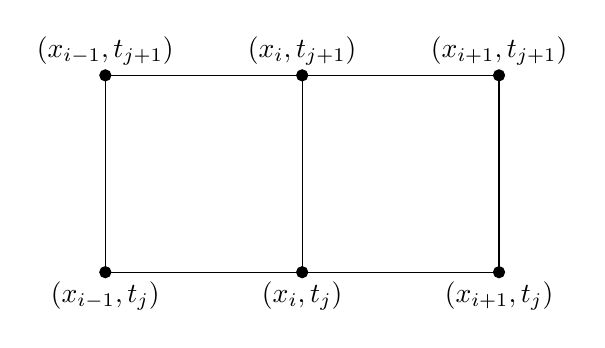
\begin{tikzpicture}
            \draw (-2.5, 0) -- (2.5, 0);
            \draw (-2.5, 2.5) -- (2.5, 2.5);
            \draw (-2.5, 0) -- (-2.5, 2.5);
            \draw (0, 0) -- (0, 2.5);
            \draw (2.5, 0) -- (2.5, 2.5);

            \filldraw[black] (-2.5, 0) circle(2pt) node[anchor=north] {$(x_{i - 1}, t_{j})$};
            \filldraw[black] (0, 0) circle(2pt) node[anchor=north] {$(x_{i}, t_{j})$};
            \filldraw[black] (2.5, 0) circle(2pt) node[anchor=north] {$(x_{i + 1}, t_{j})$};
            \filldraw[black] (-2.5, 2.5) circle(2pt) node[anchor=south] {$(x_{i - 1}, t_{j + 1})$};
            \filldraw[black] (0, 2.5) circle(2pt) node[anchor=south] {$(x_{i}, t_{j + 1})$};
            \filldraw[black] (2.5, 2.5) circle(2pt) node[anchor=south] {$(x_{i + 1}, t_{j + 1})$};
            
            % \draw (-2.5, 0) node[anchor=north] {$(x_{i - 1}, t_j)$} -- (2.5, 0) node[anchor=north] {$(x_{i + 1}, t_j)$};
            % \draw (-2.5, 2.5) node[anchor=north] {$(x_{i - 1}, t_{j + 1})$} -- (2.5, 2.5) node[anchor=north] {$(x_{i + 1}, t_{j + 1})$};
            % \draw (0, 0) -- (0, 2.5) node[anchor=south]{$(x_i, t_{j + 1})$};
            % \filldraw[black] (0, 0) circle(2pt) node[anchor=south west] {$(x_i, t_j)$};
            % \filldraw[black] (-2.5, 0) circle(2pt);
            % \filldraw[black] (2.5, 0) circle(2pt);
            % \filldraw[black] (0, 2.5) circle(2pt);
        \end{tikzpicture}
    \caption{Шеститочечный шаблон явной схемы}
    \label{fig:implicit_template}
\end{figure}
Идея неявных схем заключается в использовании шаблона, затрагивающего как значения функции на $j$--ом временном слое (который предполагается уже известным), так и на последующих слоях (значения функции на которых ещё не известны).
Так, однопараметрическое семейство неявных схем, зависящих от параметра $\sigma \in (0, 1]$ получается при аппроксимации дифференциального оператор на шеститочечном шаблоне (\seefigref{fig:implicit_template}), причём значения на \glqq верхнем\grqq и \glqq нижнем\grqq временных слоях берутся с весами $\sigma$ и $1 - \sigma$ соответственно.
Так, аппроксимация дифференциального оператора для одномерного уравнения с постоянными коэффициентами выглядит следующим образом:
\begin{multline*}
    L = \frac{\partial u}{\partial t} - \Delta u \mapsto 
    L_{h\tau} =\\
    = \frac{u_i^{j + 1} - u_i^j}{\tau} -
    \sigma\frac{u_{i + 1}^{j + 1} - 2u_i^{j + 1} + u_i^{j + 1}}{h^2}  -
    (1 - \sigma)\frac{u_{i + 1}^j - 2u_i^j + u_i^j}{h^2} + \phi_i^j,\\
    \phi_i^{j + 1} = f(x_i, t_{j + 1})
\end{multline*}
В многомерном случае можно задавать целый вектор $\sigma = (\sigma_1 \ldots \sigma_n)$:
\begin{multline*}
    L \mapsto 
    \frac{u_i^{j + 1} - u_i^j}{\tau} + \\
    + \sum\limits_{k = 1}^{n} \left[ 
        \sigma_k\frac{u_{i+}^{j + 1} - 2u_i^{j + 1} + u_{i-}^{j + 1}}{h_k^2} +
        (1 - \sigma_k) \frac{u_{i+}^j - 2u_i^j + u_{i-}^j}{h_k^2}
    \right] +\\
    + \phi_i^j,\text{ где }\\
    i_{\pm} = (i_1, \ldots, i_{k - 1}, i_k \pm 1, i_{k + 1}, \ldots, i_n)
\end{multline*}
Аналогично явной схеме, добавляя граничные и начальные условия, получаем замкнутую систему линейных уравнений.
Однако, в отличие от явной схемы, значения на новом временном слое $u^{j + 1}$ не выражаются явно через значения на предыдущем временном слое $u^{j}$, а получаются путём решения соответствующей системы линейных алгебраических уравнений $M u^{j + 1} = D$.
В одномерном случае матрица системы получается \emph{трёхдиагональной}:
\begin{equation*}
    M = \begin{pmatrix}
        B_1 & C_1 & 0 & 0 & 0 & 0 & 0\\
        A_2 & B_2 & C_2 & 0 & 0 & 0 & 0\\
        0 & A_3 & B_3 & C_3 & 0 & 0 & 0\\
        0 & 0 & A_4 & B_4 & C_4 & 0 & 0\\
        0 & 0 & 0 & \ddots & \ddots & \ddots & 0\\
        0 & 0 & 0 & 0 & A_{n-1} & B_{n-1} & C_{n-1}\\
        0 & 0 & 0 & 0 & 0 & A_{n} & B_{n}
    \end{pmatrix},
\end{equation*}
где 
\begin{align*}
    & A_i = -\sigma \tau\\
    & B_i = h^2 + 2\sigma \tau\\
    & C_i = -\sigma \tau\\
    & D_i = h^2 u_i^j + \tau (1 - \sigma) \left( 
        u_{i - 1}^j - 2u_i^j + u_{i + 1}^j
     \right) + \tau h^2 \phi_i^{j + 1}
\end{align*}
В таком случае существует эффективный алгоритм расчёта, именуемый \emph{методом прогонки}:
Сначала определяем $\alpha$ и $\beta$:
$$
    \begin{cases}
        \alpha_1 = -\frac{C_1}{B_1}, \\
        \beta_1 = \frac{D_1}{B_1}, \\
        \begin{aligned}
            & \alpha_i = -\frac{C_i}{B_i + A_i \cdot \alpha_{i-1}}\\
            & \beta_i = \frac{D_i - A_i \cdot \beta_{i-1}}{B_i + A_i \cdot \alpha_{i-1}}
        \end{aligned}, & i = 2, \ldots, n-1\\
        \beta_n = \frac{D_n - A_n \cdot \beta_{n-1}}{B_n + A_n \cdot \alpha_{n-1}}
    \end{cases}
$$
Затем по ним определяем неизвестные:
$$
    \begin{cases}
        x_n = \beta_n,\\
        x_i = \alpha_i \cdot x_{i+1} + \beta_i, & i = n-1, \ldots, 1
    \end{cases}
$$
Сложность такого алгоритма $O(N_x)$, что не уступает явной схеме.
Преимущества же неявной схемы в том, что для неё условия устойчивости принимает вид
\begin{equation*}
    \sigma \geqslant \frac{1}{2} - \frac{h^2}{4\tau}.
\end{equation*}
Из этого условия видно, что при $\sigma \ge 0.5$ схема безусловно устойчива, то есть устойчива вне зависимости от выбора шагов $h$ и $\tau$.

При значениях $\sigma \ne 0.5$ схема имеет порядок точности $O(h^2 + \tau)$, а при $\sigma = 0.5$ (так называемая \emph{схема Кранка-Николсона}) $O(h^2 + \tau^2)$, то есть больший, явная схема.

Недостатком такой схемы является отсутствие возможности распараллеливания.

В случае многомерной задачи дело обстоит хуже.
Получаемые системы линейных уравнений имеют более сложную матрицу (не трёхдиагональную). Для их решения пользуются в общем случае методом последовательного исключения переменных (методом Гаусса), который работает за $O(N^3)$, где $N \times N$~--- размерность матрицы.
Так, уже в двумерной задаче матрица будет размера $N_xN_y \times N_x N_y$, и расчёт будет проводиться заметно дольше, чем при расчёте явной схемой ($\sim O(N^2)$).
            % Локально-одномерные схемы
            \subsubsection{Локально-одномерные схемы}
            \newcommand{\valpha}{v_{(\alpha)}}

Итак, явные схемы обладают быстрой скоростью счёта ($\sim O(N^n)$), в то время как устойчивость таких систем достигается лишь при определённом выборе параметров сетки.
Неявные схемы безусловно устойчивы и имеют больший порядок точности, однако требуют решения системы $N^n$ уравнений, для чего требуется значительно больше вычислительной работы, чем для явной схемы \cite{ТихоновСамарский}.

Для сочетания лучших качеств явных (объём работы $\sim O(N^n)$) и неявных (безусловная устойчивость) схем было предложено несколько \emph{экономичных} схем.
Подбробнее об этом написано в \cite{СамарскийТеорияРазностныхСхем, peaceman1955numerical, douglas1955numerical, яненко1959одном, дьяконов1962разностные, самарский1962одном}.

\emph{Локально-одномерный метод} является универсальным, пригодным для решения квазилинейного уравнения теплопроводности в произвольной области $G$ любого числа измерений.
При использовании в работе блочных локально-адаптивных сеток (раздел \ref{sec:LAG}) используется именно этот метод.
Также будут использоваться прямоугольные области, поэтому формулировка метода будет приведена для таковых.

Итак, рассматриваемую многомерную задачу Дирихле в цилиндре $\bar{Q}_T = \bar{G} \times [0, T]$, $\bar{G} = \prod\limits_{i=1}^{n} [0, L_i]$
\begin{equation*}
    \begin{aligned}
        &\left\{ 
            \begin{aligned}
                & u_t = \sum\limits_{\alpha = 1}^{p} \frac{\partial }{\partial x_{\alpha}} \left[ 
                    k_{\alpha}(u) \frac{\partial u}{\partial x_{\alpha}}
                 \right] + f, && (x, t) \in G \times (0, T]\\
                & \begin{aligned}
                    & u(x, t) = \mu_{-i}(x, t), && x_i = 0\\
                    & u(x, t) = \mu_{i}(x, t), && x_i = L_i
                \end{aligned}, && t \in [0, T)\\
                &u(x, 0) = u_0(x), && x \in \bar{G}
            \end{aligned}
        \right.\\
    \end{aligned}
\end{equation*}
заменяем \emph{цепочкой одномерных} задач \glqq вдоль каждого из напарвлений\grqq:
\begin{equation*}
    \begin{cases}
        \frac{1}{p} \frac{\partial v_{(\alpha)}}{\partial t} = \frac{\partial }{\partial x_{\alpha}} \left[ k_{\alpha}(v_{(\alpha)}) \frac{\partial v_{(\alpha)}}{\partial x_{\alpha}} \right] + f_{\alpha}, &
            x \in G, t \in \Delta_{\alpha} = \left( 
                t_{j + \frac{\alpha - 1}{p}}, 
                t_{j + \frac{\alpha}{p}}
            \right]\\
        \valpha(x, t_{j + \frac{\alpha - 1}{p}}) = v_{(\alpha - 1)}(x, t_{j + \frac{\alpha - 1}{p}}), & x \in G\\
        \valpha(x, t) = \mu_{-\alpha}(x, t), & x_{\alpha} = 0, t \in [t_{j + \frac{\alpha - 1}{p}}, t_{j + \frac{\alpha }{p}}]\\
        \valpha(x, t) = \mu_{\alpha}(x, t), & x_{\alpha} = L_{\alpha}, t \in [t_{j + \frac{\alpha - 1}{p}}, t_{j + \frac{\alpha }{p}}]\\
    \end{cases}
\end{equation*}
\begin{equation*}
    \begin{aligned}
        &\valpha(x, 0) = u_0(x)\\
        & v_{(1)}(x, t_j) = v_{(p)}(x, t_j)\\
        & u(x, t_{j + 1}) = v_{(p)}(x, t_{j + 1}).
    \end{aligned}
\end{equation*}
Каждая из одномерных задач решается неявной двухслойной схемой:
\begin{multline*}
    \frac{v_{(\alpha)}^{j + \frac{\alpha}{p}} - v_{(\alpha)}^{j + \frac{\alpha - 1}{p}}}{\tau} =
    \frac{1}{h_{\alpha}^2} \left[ 
        a_{i_{\alpha} + 1}^{(\alpha)} \left( v_{(\alpha)}^{j + \frac{\alpha - 1}{p}} \right) \cdot \left( 
            v_{(\alpha)i_{\alpha} + 1}^{j + \frac{\alpha}{p}} - v_{(\alpha)i_{\alpha}}^{j + \frac{\alpha}{p}}
         \right)-\right.\\
         \left. - a_{i_{\alpha}}^{(\alpha)} \left(v_{(\alpha)}^{j + \frac{\alpha - 1}{p}}\right) \cdot \left( 
             v_{(\alpha), i_{\alpha}}^{j + \frac{\alpha}{p}} - v_{(\alpha), i_{\alpha} - 1}^{j + \frac{\alpha}{p}}
          \right)
     \right] + f_{\alpha} \left( 
         v_{(\alpha)}^{j + \frac{\alpha - 1}{p}}
      \right), \\
      \text{ где } a_i^{(\alpha)} (y) = k_{\alpha} \left( \frac{y_{i - 1} + y_i}{2} \right), \quad 
      i_{\alpha} \pm 1 = (i_1, \ldots, i_{\alpha - 1}, i_{\alpha} \pm 1, i_{\alpha + 1}, \ldots, i_{p})
\end{multline*}

Напишем подробнее, как выглядит данная схема в случае двумерного квазилинейного уравнения теплопроводности.
Цилиндр $\bar{Q}_T = [0, L_1] \times [0, L_2] \times [0, T]$ дискретизуется равномерной сеткой:
\begin{multline*}
    \omega_{h\tau} = \left\{ 
        (x_i, y_k, t_j) \mid x_i = h_x \cdot (i - 1), y_k = h_y \cdot (k - 1), t_j = \tau \cdot (j - 1),\right.\\
        \left. i = 1,\ldots,N_x,\quad k = 1,\ldots, N_y, \quad j = 1, \ldots, N_t
     \right\}
\end{multline*}
Исходная задача с уравнением
\begin{equation*}
    \frac{\partial u}{\partial t} = \frac{\partial}{\partial x}\left( k_1(u) \frac{\partial u}{\partial x} \right) +
    \frac{\partial}{\partial y} \left( k_2(u) \frac{\partial u}{\partial y} \right) + f
\end{equation*}
заменяется на две одномерные задачи, каждая из которых решается неявной схемой.
Обозначим $w := u^{j + 1/2}$~--- промежуточное значение, получающееся при решении первой из задач на интервале времени $(t_{j}, t_{j + 1/2})$ (вдоль оси $x_1$).
Решение в начальный момент времени $t_1 = 0$ известно из начальных данных:
\begin{equation*}
    u_{i, k}^{1} = u_0(x_i, y_k)\quad \forall i, k
\end{equation*}
Зная решение на $j$--ом временном слое $u_{i, k}^{j}$, решение на $(j + 1)$--ом ищется следующим образом:
сначала решается $N_y$ одномерных задач вдоль оси $x$ ($N_y$~--- для каждого $y_k, k = 1,\ldots,N_y$ независимо):
\begin{equation*}
    \begin{cases}
        \begin{aligned}
            \textstyle\frac{w_{i, k} - u_{i, k}^{j}}{\tau} = &\textstyle \frac{1}{h_x^2} \left[ 
                k_1 \left( 
                    \frac{u_{i, k}^{j} + u_{i + 1, k}^{j}}{2}
                \right) \cdot \left( 
                    w_{i + 1, k} - w_{i, k}
                \right) -
            \right.\\
            &\textstyle \left.
                - k_1 \left( 
                    \frac{u_{i - 1, k}^{j} + u_{i, k}^{j}}{2}
                \right) \cdot \left( 
                    w_{i, k} - w_{i - 1, k}
                \right)
            \right] + \frac{1}{2}\phi_{i, k}^{j + 1/2}
        \end{aligned}, & i = 2, \ldots, N_x - 1\\ 
        w_{1, k} = \mu_{-1}(y_k, t_{j + 1/2})\\
        w_{N_x, k} = \mu_{1}(y_k, t_{j + 1/2})
    \end{cases}
\end{equation*}
Затем решается $N_x$ одномерных задач вдоль оси $y$ ($N_x$~--- для каждого $x_i, i = 1, \ldots, N_x$ независимо):
\begin{equation*}
    \begin{cases}
        \begin{aligned}
            \textstyle\frac{u_{i, k}^{j + 1} - w_{i, k}}{\tau} = &\textstyle \frac{1}{h_y^2} \left[ 
                k_2 \left( 
                    \frac{w_{i, k} + w_{i, k + 1}}{2}
                \right) \cdot \left( 
                    u_{i, k + 1}^{j + 1} - u_{i, k}^{j + 1}
                \right) -
            \right.\\
            &\textstyle \left.
                k_2 \left(
                    \frac{w_{i, k - 1} + w_{i, k}}{2}
                \right) \cdot \left( 
                    u_{i, k}^{j + 1} - u_{i, k - 1}^{j + 1}
                \right)
            \right] + \frac{1}{2}\phi_{i, k}^{j + 1}, 
        \end{aligned} & k = 2, \ldots, N_y - 1\\
        u_{i, 1}^{j + 1} = \mu_{-2}(x_i, t_{j + 1})\\
        u_{i, N_y}^{j + 1} = \mu_2(x_i, t_{j + 1})
    \end{cases}
\end{equation*}
Каждая из одномерных задач решается методом прогонки за $O(N)$, где $N = N_x, N_y$.
И, таким образом, общая сложность такого алгоритма есть $O(N_y \cdot N_x + N_x \cdot N_y) = O(N^2)$, то есть совпадает по скорости решения с явной схемой.

В многомерном случае область $G$ дискретизуется сеткой $\omega_h$, имеющий вдоль каждого направления $N$ точек.
Для каждого значения $\alpha = 1, \ldots, p$ получается $N^{p - 1}$ задач. 
Каждая из них решается методом прогодки за $\sim O(N)$ и, таким образом, число арифметиеских операций, совершаемых в локально-одномерной схеме есть число порядка $\sim O(N^p)$.
Помимо быстрой скорости счёта, ЛОС обладает и существенным достоинством неявных схем.
Как показано в \cite{СамарскийТеорияРазностныхСхем}, схема аппроксимирует исходное уравнение в суммарном смысле:
погрешность аппроксимации $\psi$ для локально-одномерной схемы есть сумма погрешностей аппроксимации $\psi_{\alpha}$ на решении $u = u(x, t)$ для одномерных схем номера $\alpha$:
\begin{equation*}
    \psi = \sum_{\alpha = 1}^{p} \psi_{\alpha} = O(|h|^2 + \tau),
\end{equation*}
ЛОС безусловно устойчива и равномерно сходится.
Это означает, что счёт по данной схеме устойчив даже при очень крупных шагах по времени, что позволяет быстро решать задачи, где не требуется большая точность.

Помимо прочего стоит отметить, что данный метод применим не только к параллелепипедам, но и к произвольным областям $G \subset \mathbb{R}^{p}$, сохраняет порядок точности на неравномерных сетках \cite{СамарскийНеравномерныеСетки}, обладает пониженными (по сравнению с другими схемами) требованиями к объёму перативной памяти, а также допускает распараллеливание: вдоль каждого из напарвлений необходимо решать $N$ систем линейных уравнений, и все они могут решаться независимо друг от друга и, следовательно, параллельно.

Учитывая все преимущества локально-одномерной схемы для уравнения теплопроводности, именно она берётся в основу при рассмотрении локально-адаптивных сеток в разделе \ref{sec:LAG}.
        % Программный код, примеры расчётов
        \subsection{Программный код, примеры расчётов}\label{sec:StaticCode}
    
    % Теория блочных локально-адаптивных сеток
    \section{Теория блочных локально-адаптивных сеток}\label{sec:LAG}
    
    % Замечаения о программной реализации
    \section{Замечания о программной реализации}

    % Основные результаты
    \section{Основные результаты}

    % Приложения к физике, реальные задачи
    \section{Приложения к физике, реальные задачи}

    % Заключение
    \section{Заключение}

    % Список Литературы
    \newpage
    \renewcommand{\refname}{Список литературы}
    \printbibliography
    \addcontentsline{toc}{section}{\refname}
\end{document}